\section{Feedback-Optimized Reliable Consensus Sampling}
For CS and RCS, the framework does not require an explicit definition of security properties. This design allows algorithms to remain applicable over time. From this perspective, for each concrete task, one cannot determine the probability that the final delivered result is safe. This holds even though the algorithmic risk admits an upper bound. External control over the sampling process is limited. This implies that, from both an algorithmic and long-term operational perspective, if the $\mathcal{MG}$ remains unchanged and the input task types are essentially fixed, the risk in RCS remains stationary over time, thereby limiting the potential for dynamic optimization. In this section, we analyze the nature of response safety in RCS. Inspired by quantum computing \citep{nielsen2010quantum}, we propose a research methodology for RCS based on quantum states. We further introduce a mechanism that intervenes in model distributions and dynamically improves safety.


\subsection{Foundational Theory}
\label{sec:Theory}
\noindent
Motivated by quantum computation theory, we propose a framework for studying the security of RCS by analogy with quantum theory.

\noindent
\textbf{Understanding RCS Safety from a Quantum State Perspective}. 
We model a system with unknown safety as a quantum state $|\phi\rangle$, defined as
$|\phi\rangle = \alpha |0\rangle + \beta |1\rangle$,
where $|0\rangle$ denotes a safe state and $|1\rangle$ denotes an unsafe state. The constraint $\alpha^2 + \beta^2 = 1$ holds. Before evaluation, $|\phi\rangle$ does not reside in a definite safe or unsafe state. It remains in a superposition, analogous to Schr\"odinger's cat. The value $|\alpha|^2$ denotes the probability of safety, while $|\beta|^2$ denotes the probability of unsafety.

Given a fixed prompt $q$ and an evaluation method $e$, we apply $\mathrm{Eval}(q, |\phi\rangle, e)$. The state $|\phi\rangle$ then collapses to $|0\rangle$ or $|1\rangle$. Only at this stage can one determine safety under $q$ and $e$. Therefore, $|\phi\rangle$ alone cannot be labeled as safe or unsafe. The state becomes concrete only under the joint action of $q$ and $e$. The desired condition is $|\alpha| > |\beta|$, meaning a stronger bias toward the safe state.

\noindent
\textbf{Entanglement Theory for RCS}. Consider an $\mathcal{MG}$ with $n$ models $\{|\phi_1\rangle, |\phi_2\rangle, \dots, |\phi_n\rangle\}$. In each sampling round, the randomly selected model $|\phi_r\rangle$ remains in a superposition of safety and unsafety. However, the response $y$ produced by $|\phi_r\rangle$ implicitly links $|\phi_r\rangle$ with other models. In $\mathcal{MG}$, there exists a subset
$W = \{|\phi_1\rangle, |\phi_2\rangle, \dots, |\phi_\ell\rangle\}$
that assigns a high probability to $y$. There also exists a subset
$X = \{|\phi_{\ell+1}\rangle, |\phi_{\ell+2}\rangle, \dots, |\phi_n\rangle\}$
that assigns a low probability to $y$. The model $|\phi_r\rangle$ belongs to neither $W$ nor $X$. We say that $W$ and $X$ are entangled. After a time interval $\Delta(t)$, suppose evaluation under $q$ and $e$ verifies that $|\phi_r\rangle$ is unsafe. Then models in $W$ are likely unsafe, while models in $X$ are likely safe. In subsequent sampling, when a prompt $x$ and an evaluation $a$ resemble $q$ and $e$, the algorithm should increase weights for models in $X$ and decrease weights for models in $W$.






\begin{figure*}[!]
    \centering
    \begin{subfigure}{0.31\textwidth}
        \centering
        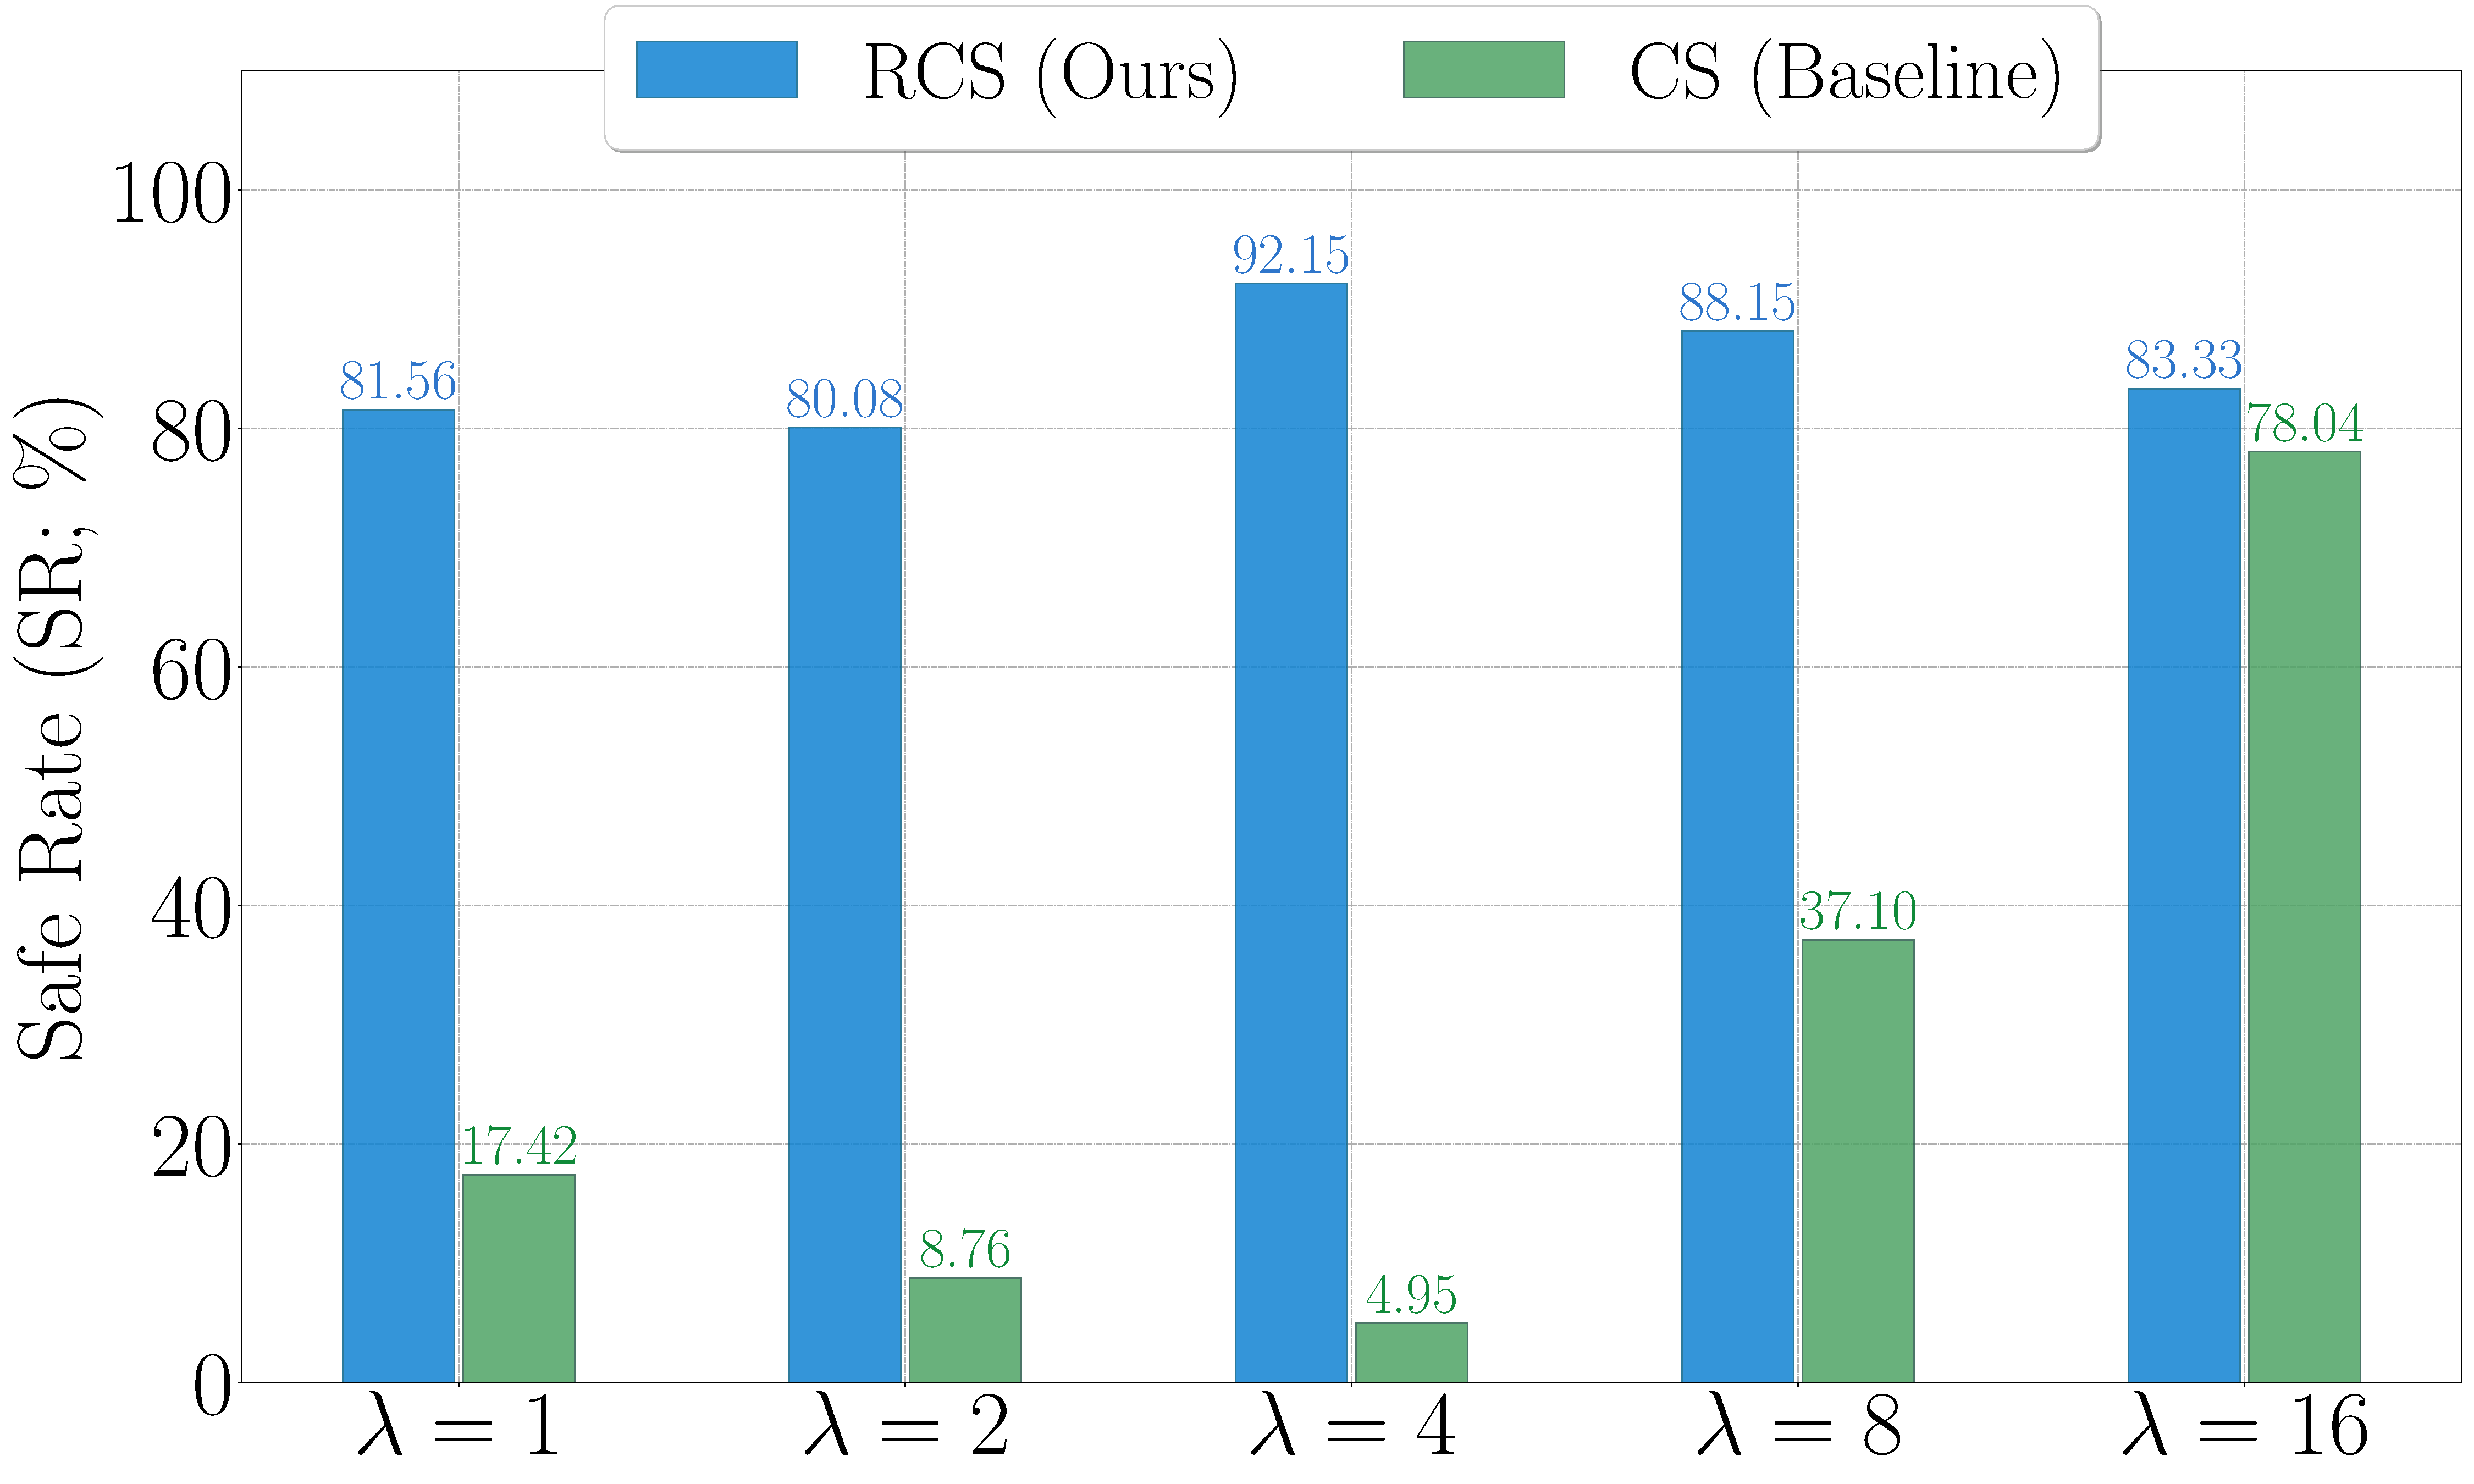
\includegraphics[width=\linewidth]{latex/eval_res/SR-33.pdf}
        \caption{$n=33$.}
    \end{subfigure}
    \begin{subfigure}{0.31\textwidth}
        \centering
        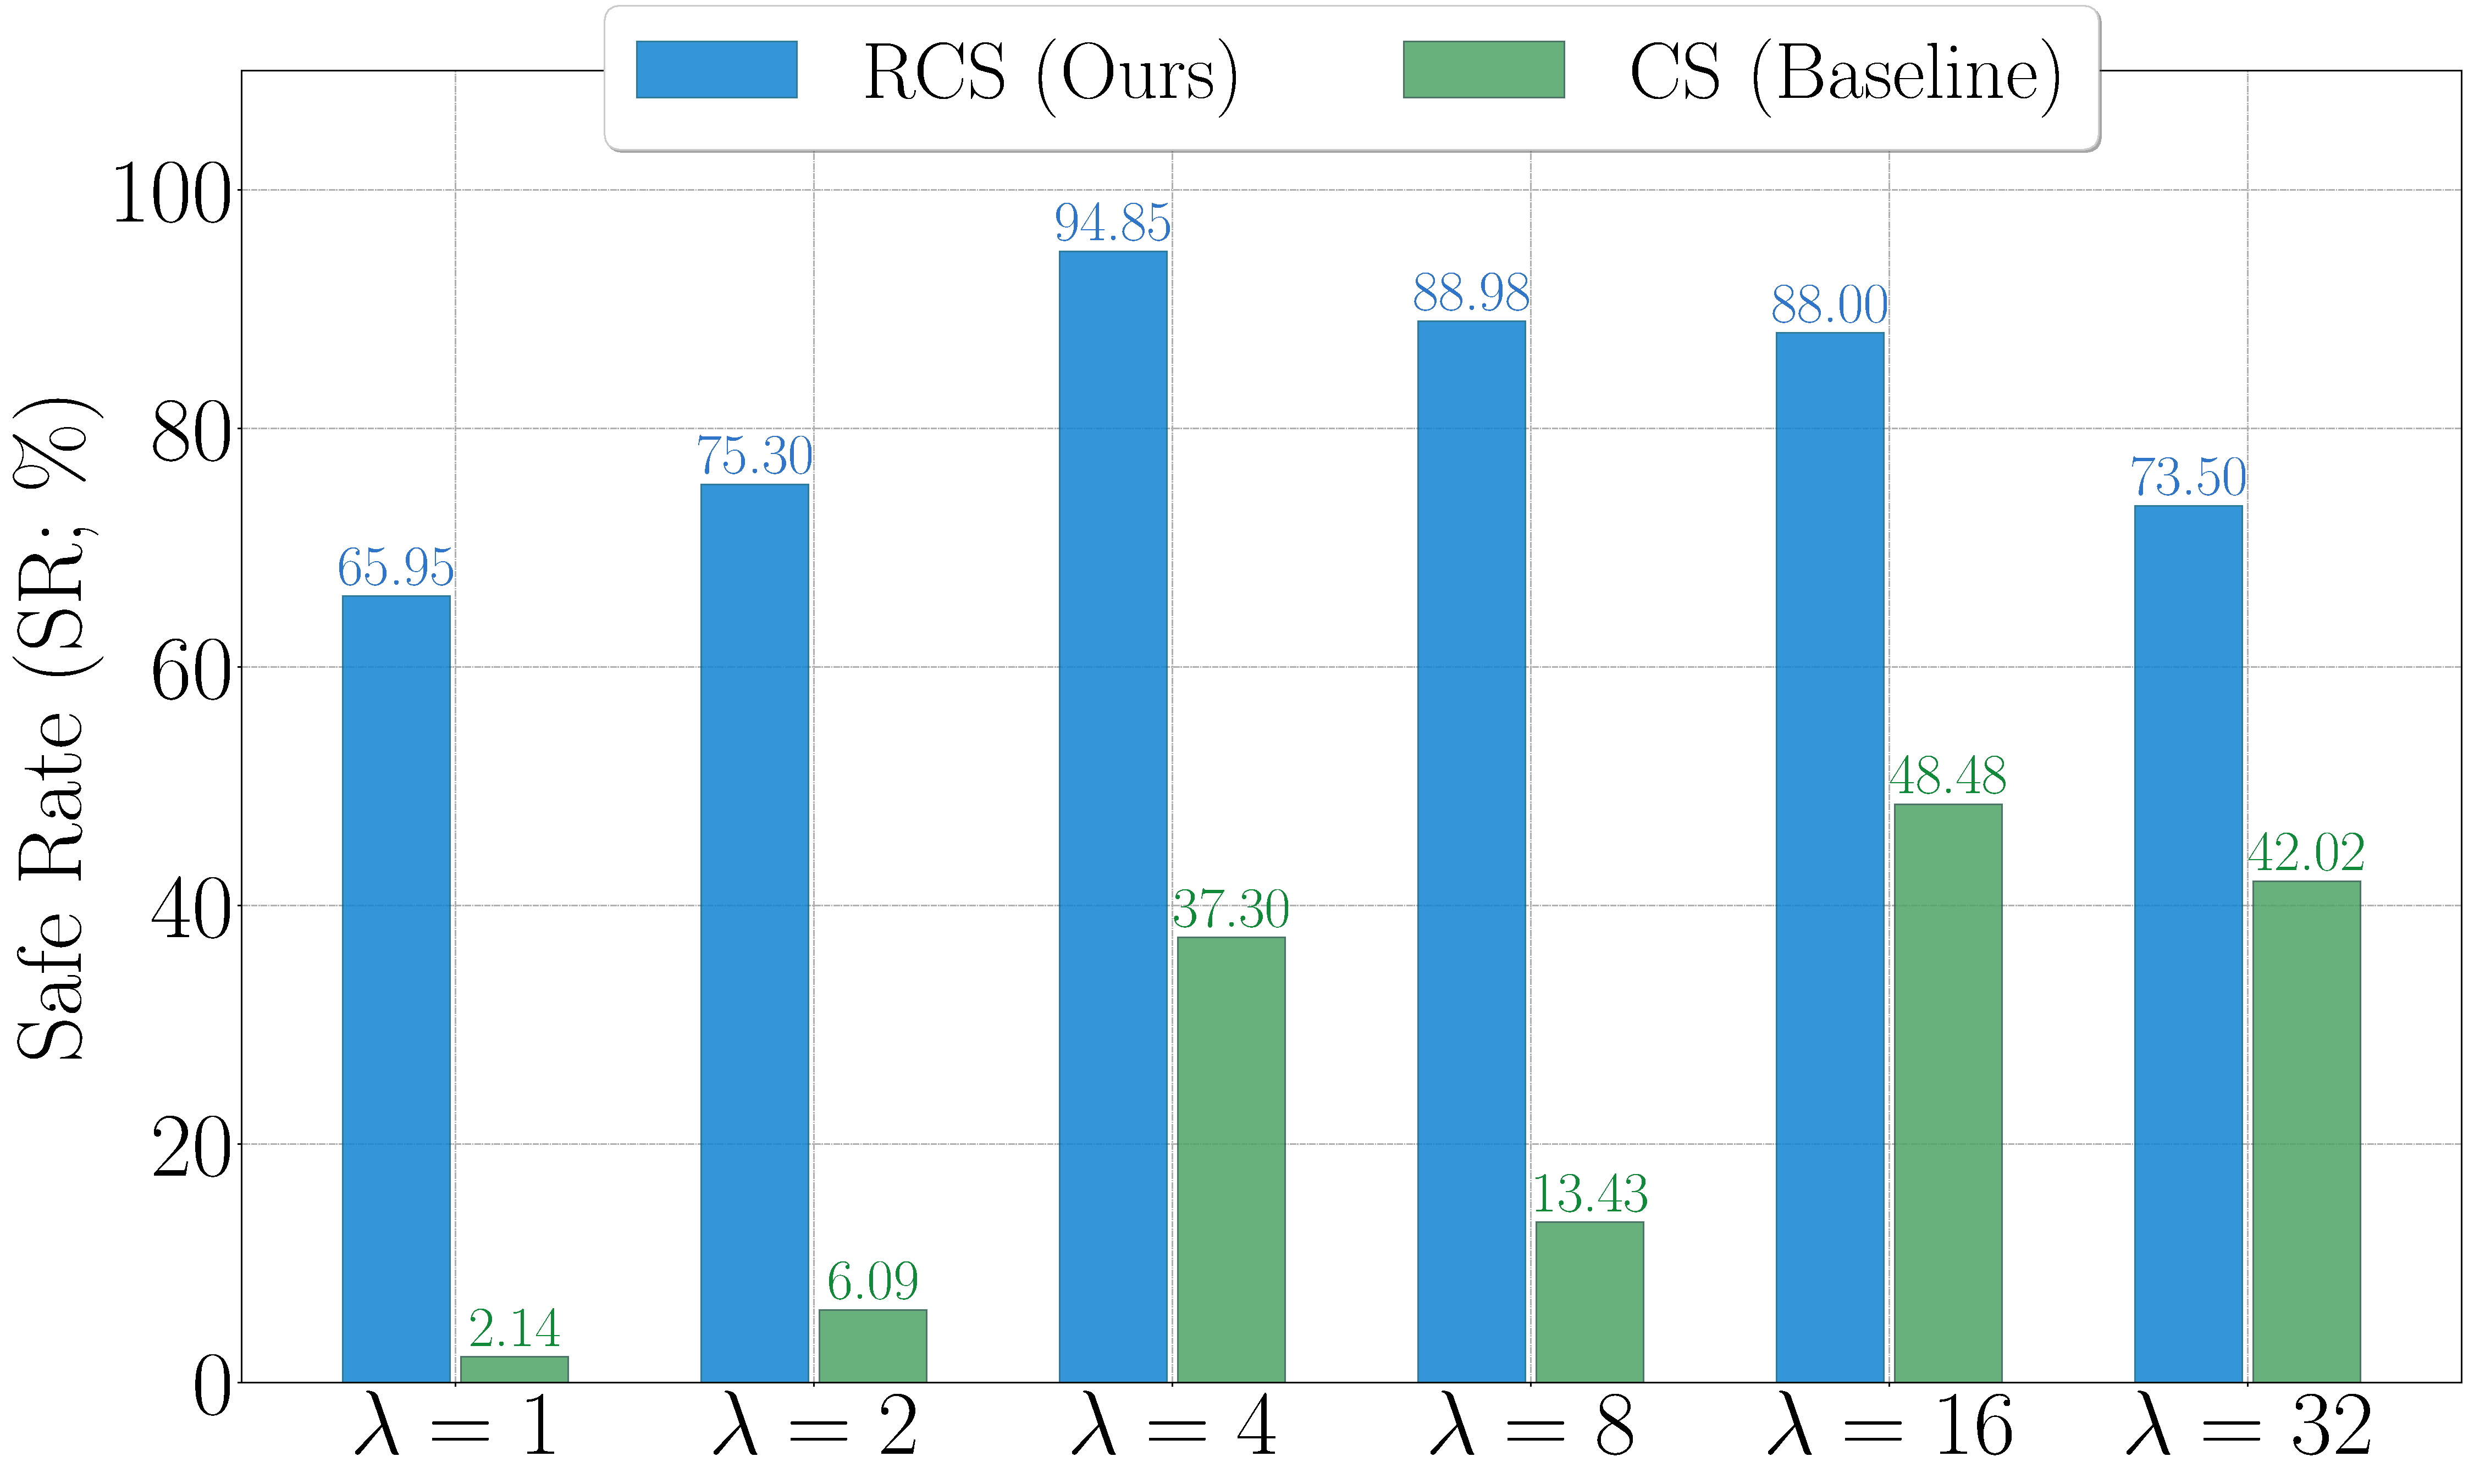
\includegraphics[width=\linewidth]{latex/eval_res/SR-65.pdf}
        \caption{$n=65$.}
    \end{subfigure}
    \begin{subfigure}{0.31\textwidth}
        \centering
        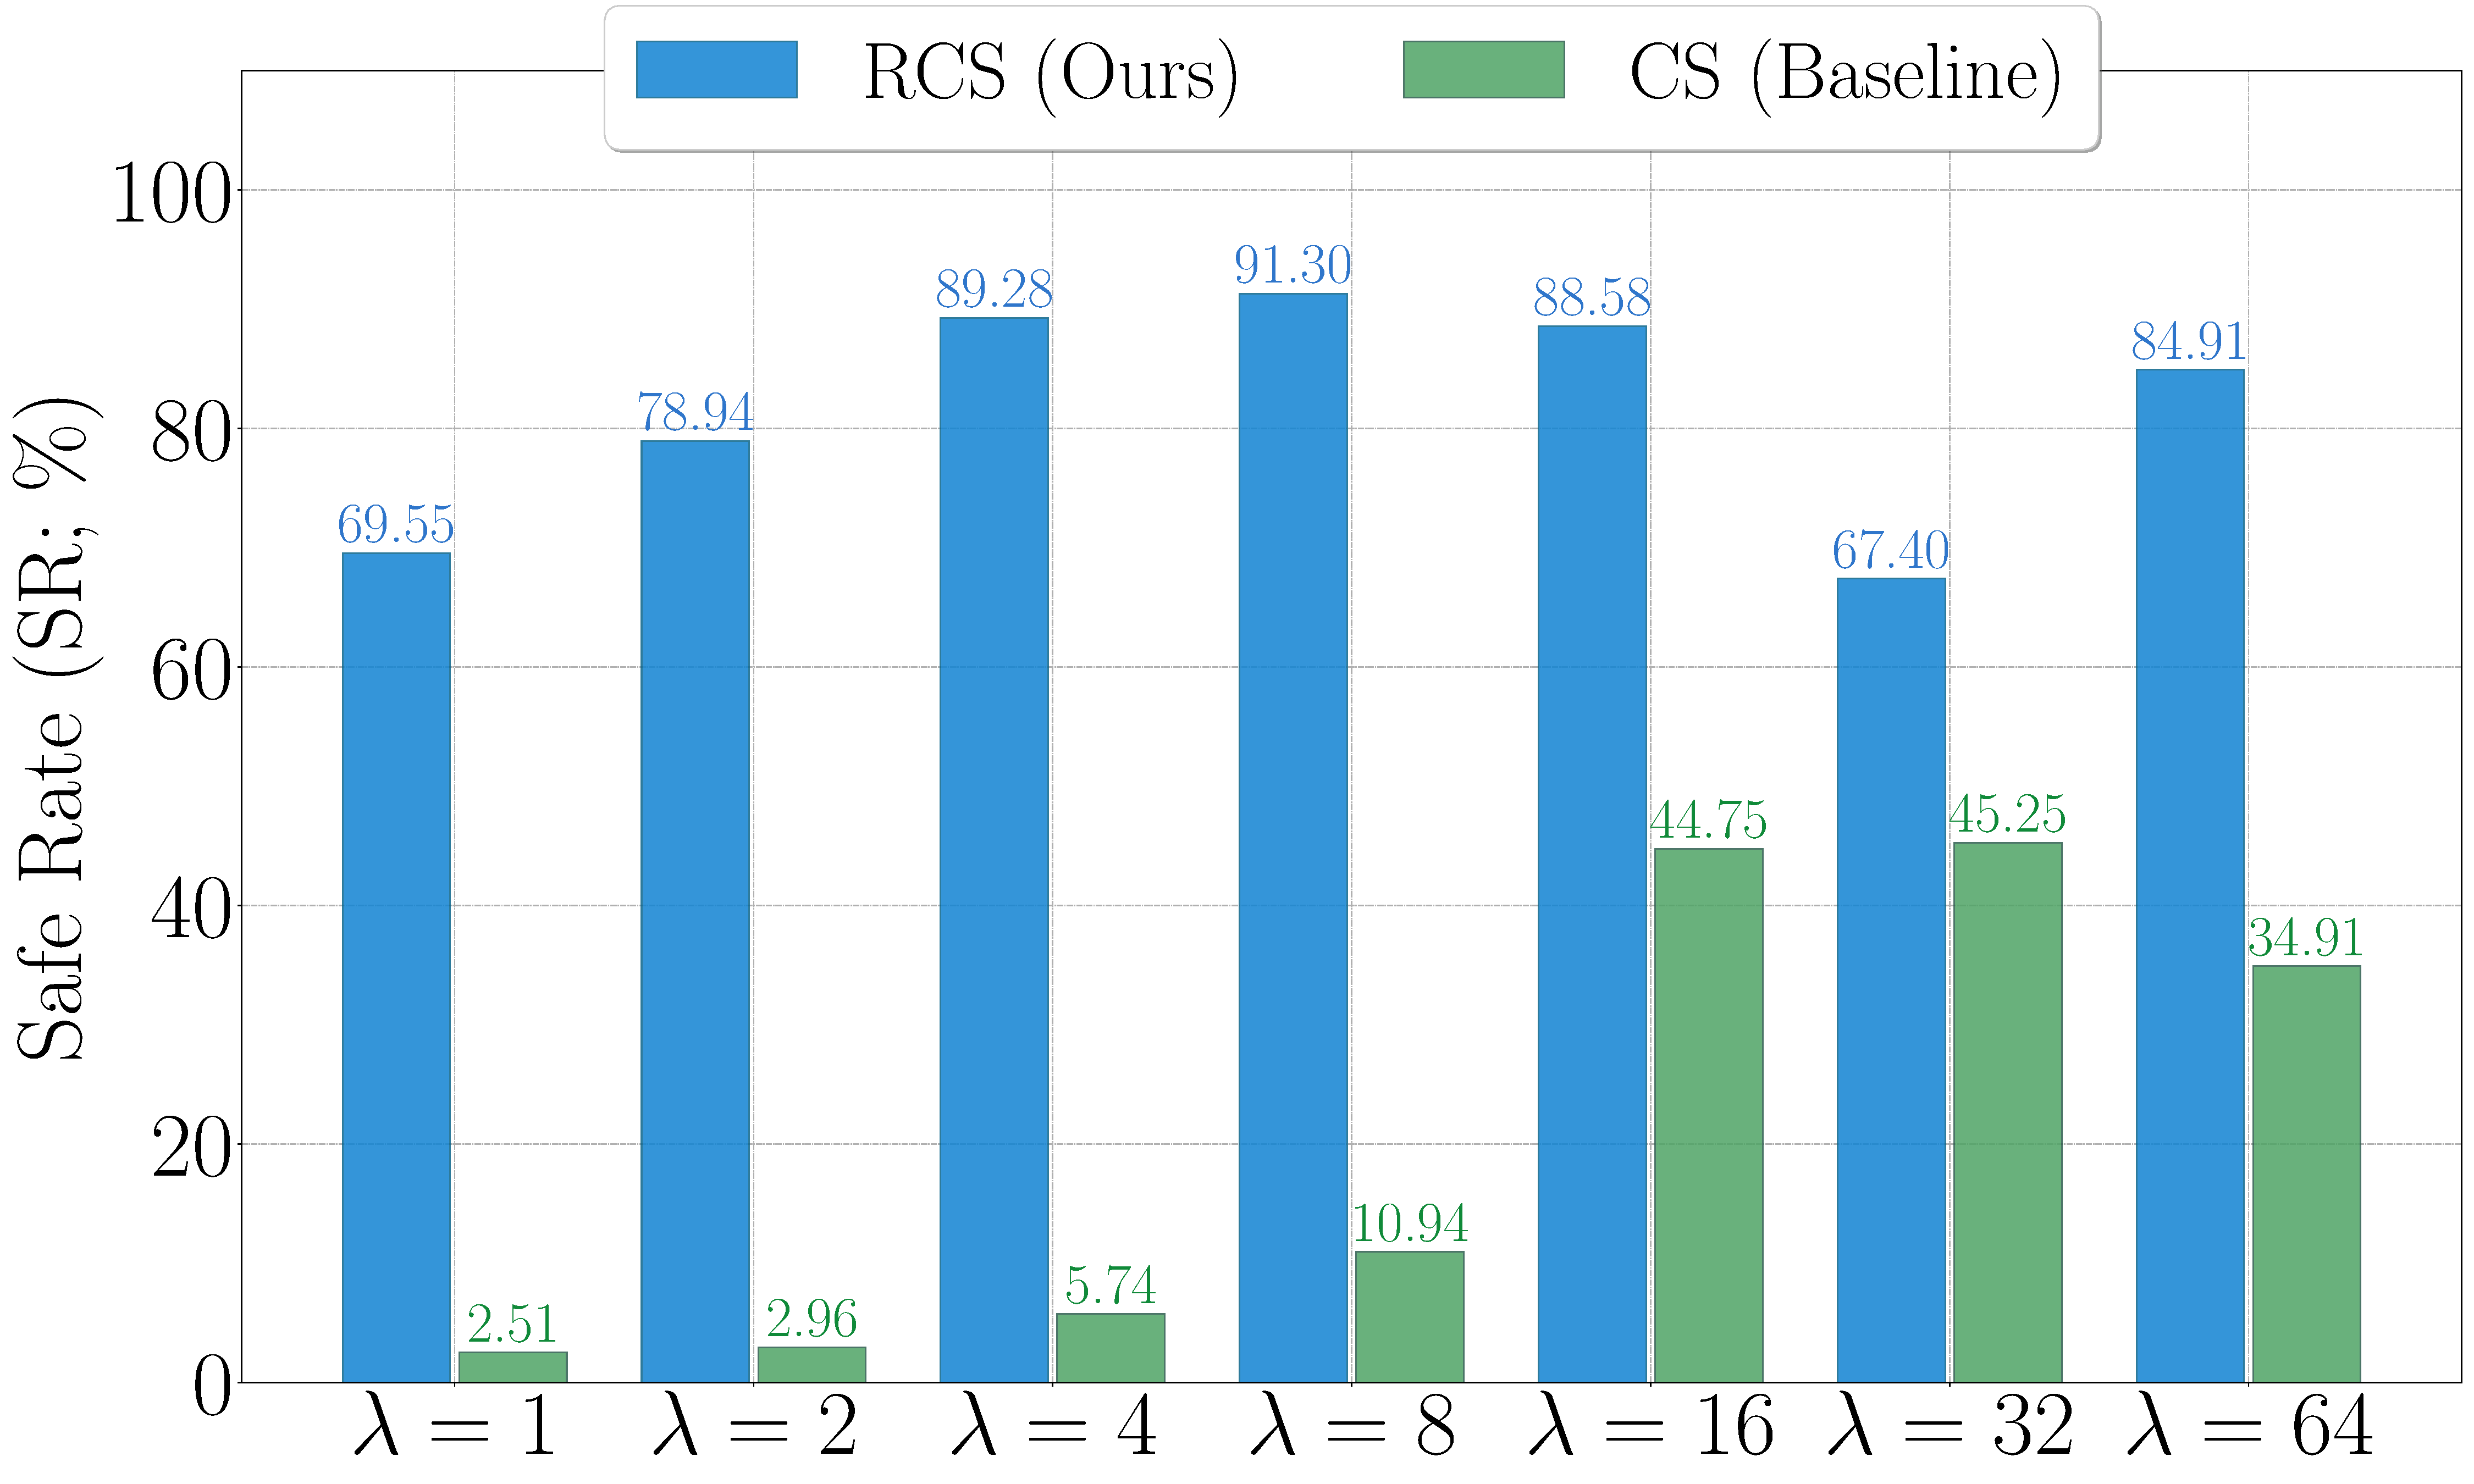
\includegraphics[width=\linewidth]{latex/eval_res/SR-129.pdf}
        \caption{$n=129$.}
    \end{subfigure}
    \caption{Evaluation results for the safe rate when $f < \lceil \frac{n}{2} \rceil$.}
    \label{fig:SR_g}
    % \vspace{-15pt}
\end{figure*}



\begin{figure*}[!]
    \centering
    \begin{subfigure}{0.31\textwidth}
        \centering
        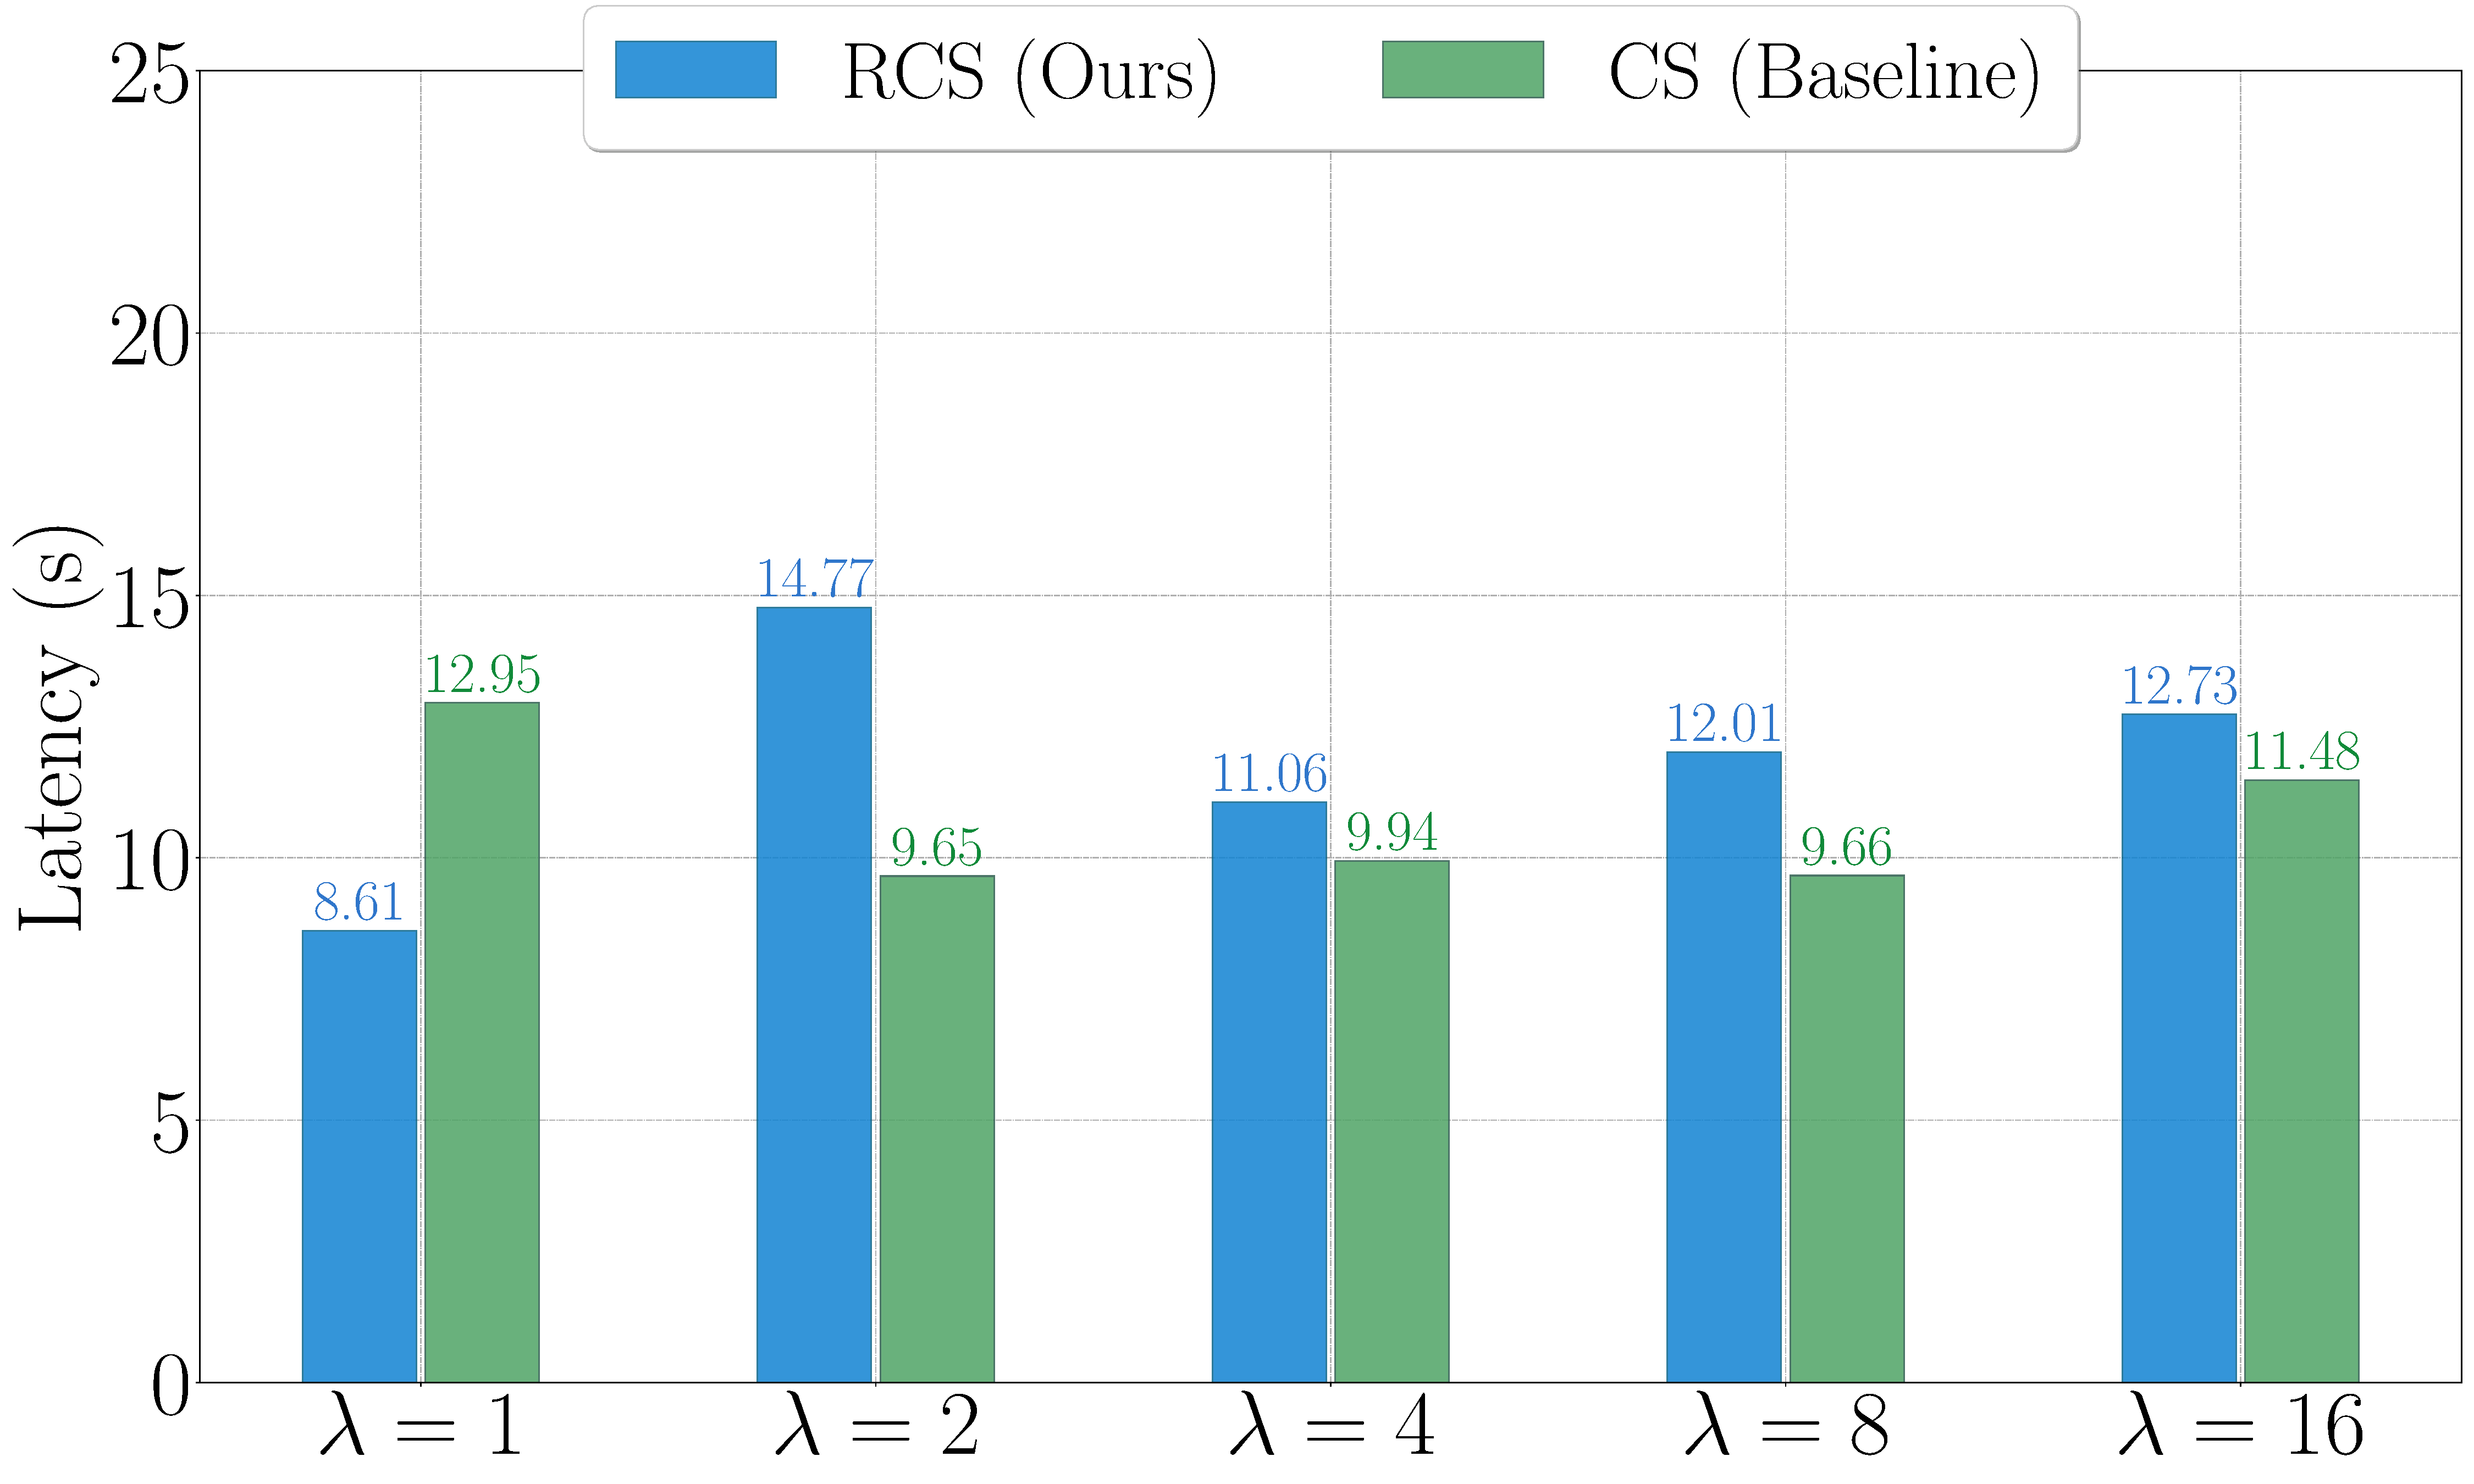
\includegraphics[width=\linewidth]{latex/eval_res/TC-33.pdf}
        \caption{$n=33$.}
    \end{subfigure}
    \begin{subfigure}{0.31\textwidth}
        \centering
        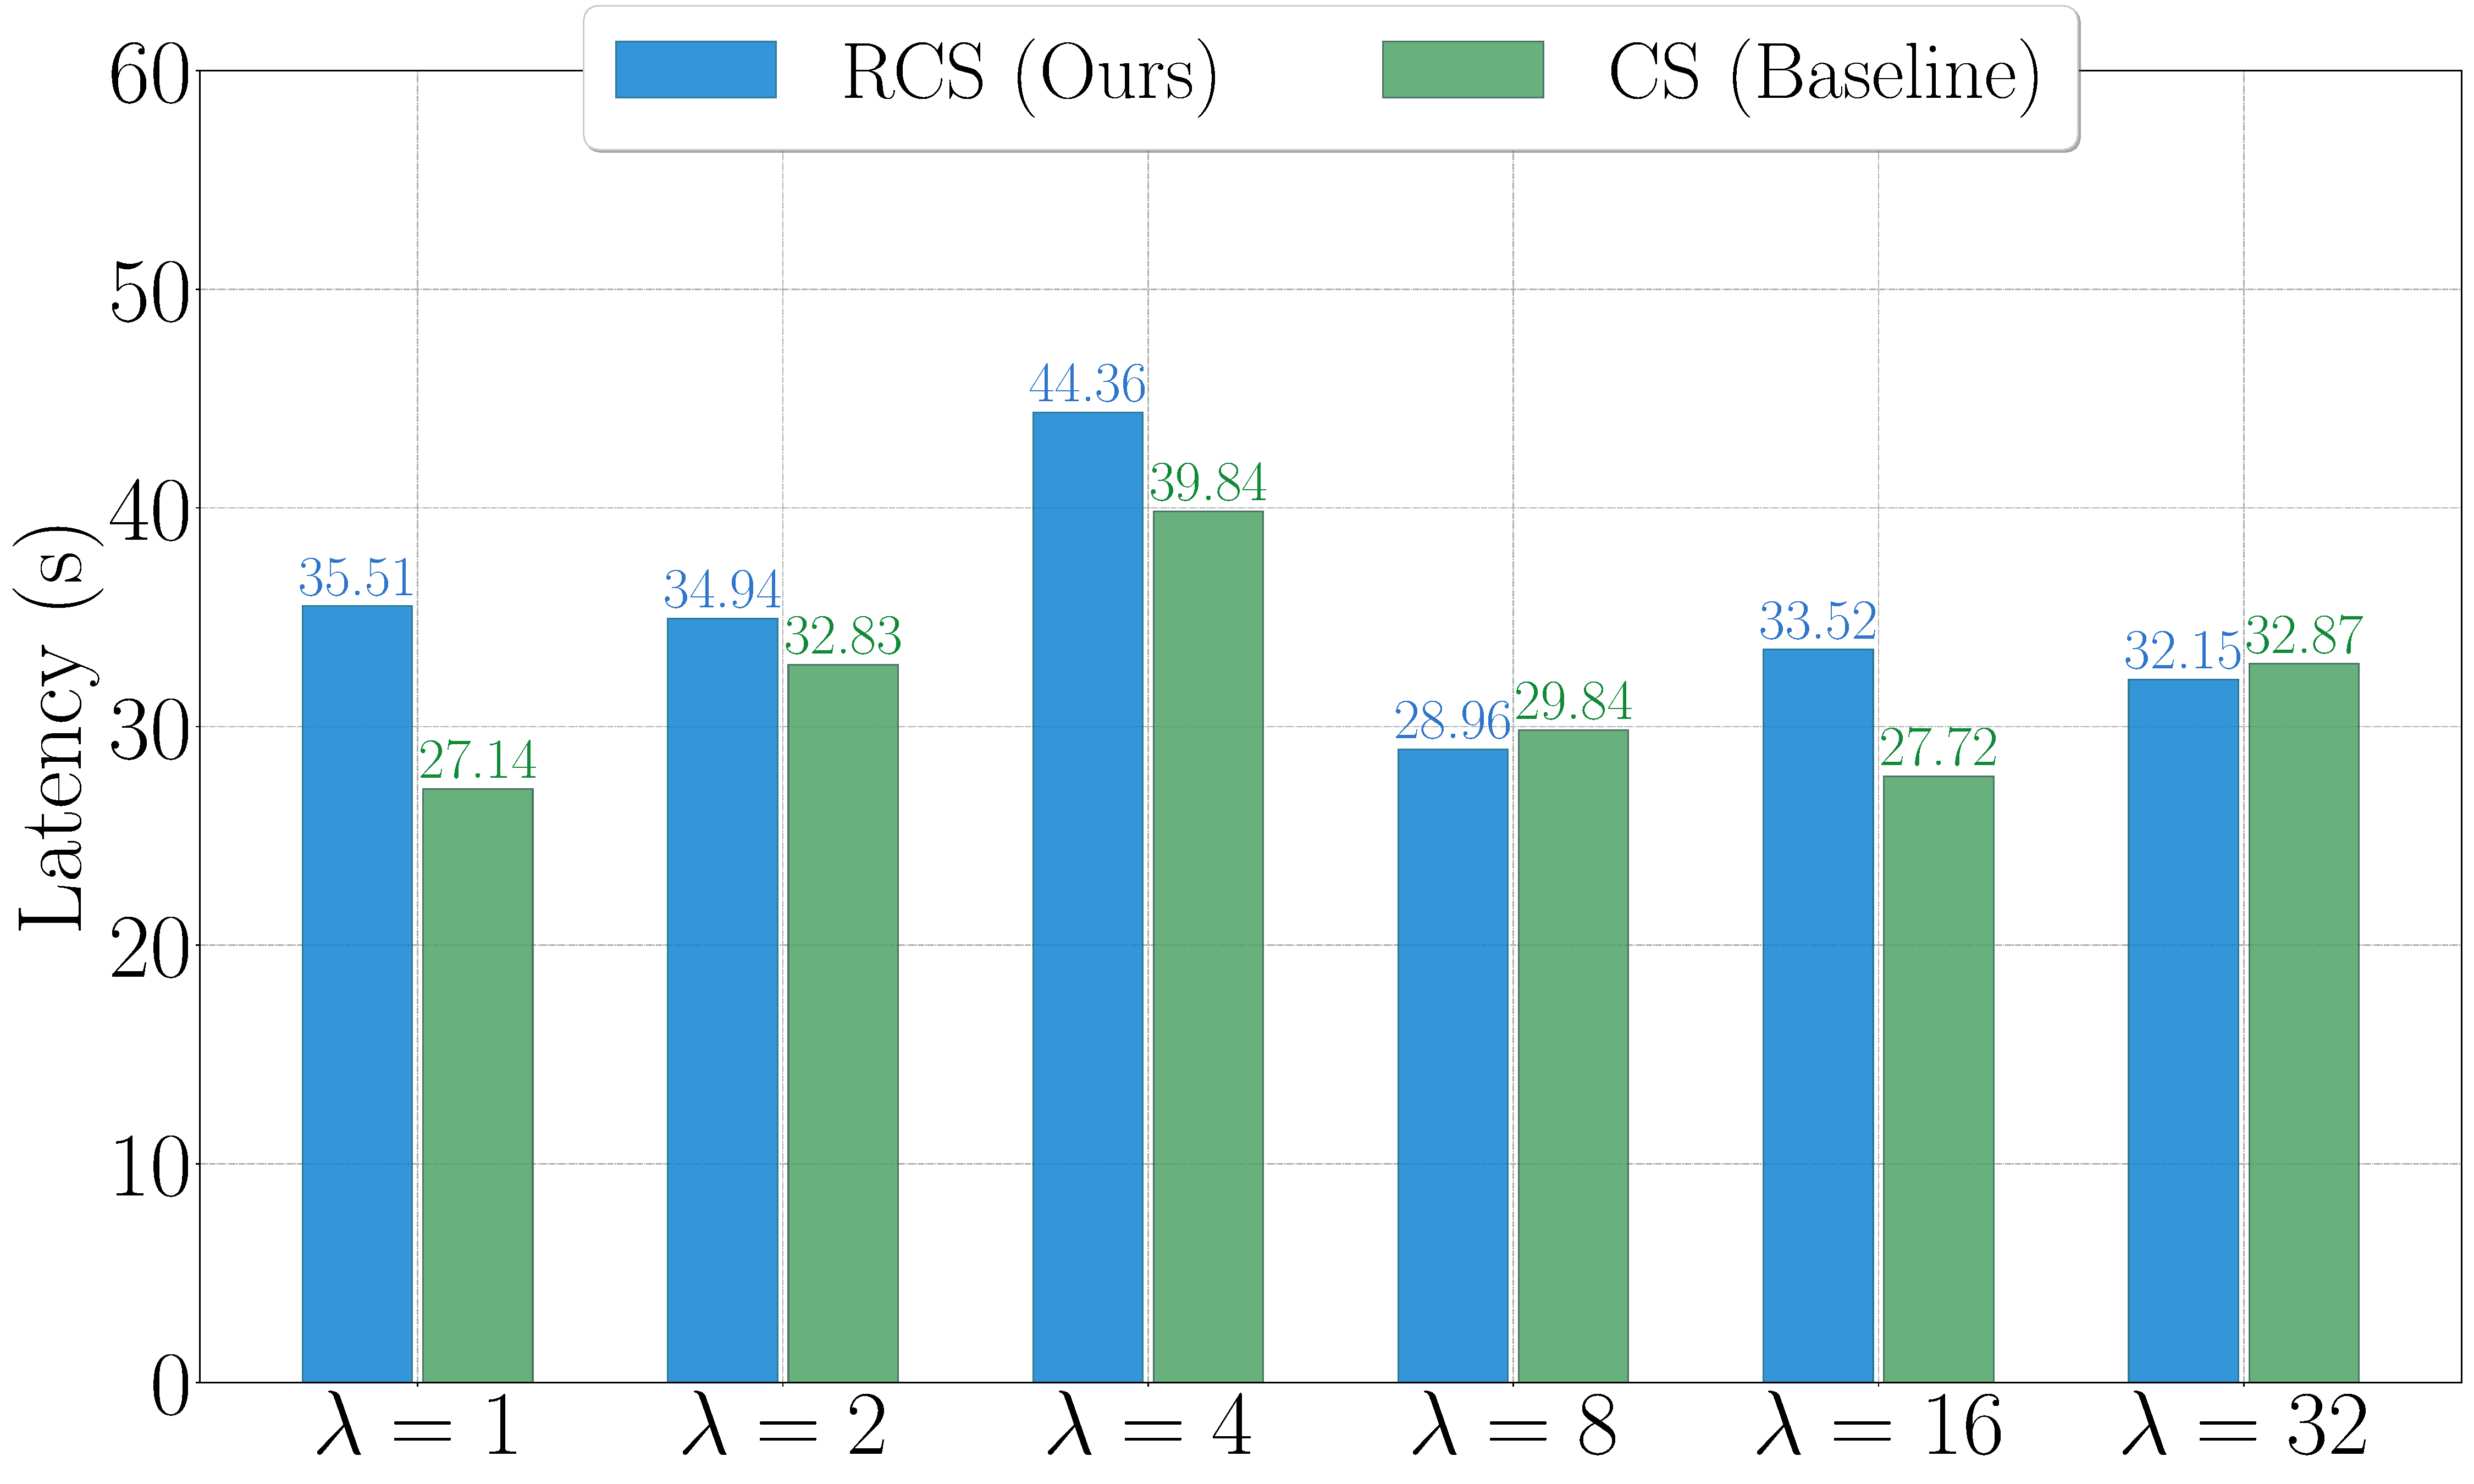
\includegraphics[width=\linewidth]{latex/eval_res/TC-65.pdf}
        \caption{$n=65$.}
    \end{subfigure}
    \begin{subfigure}{0.31\textwidth}
        \centering
        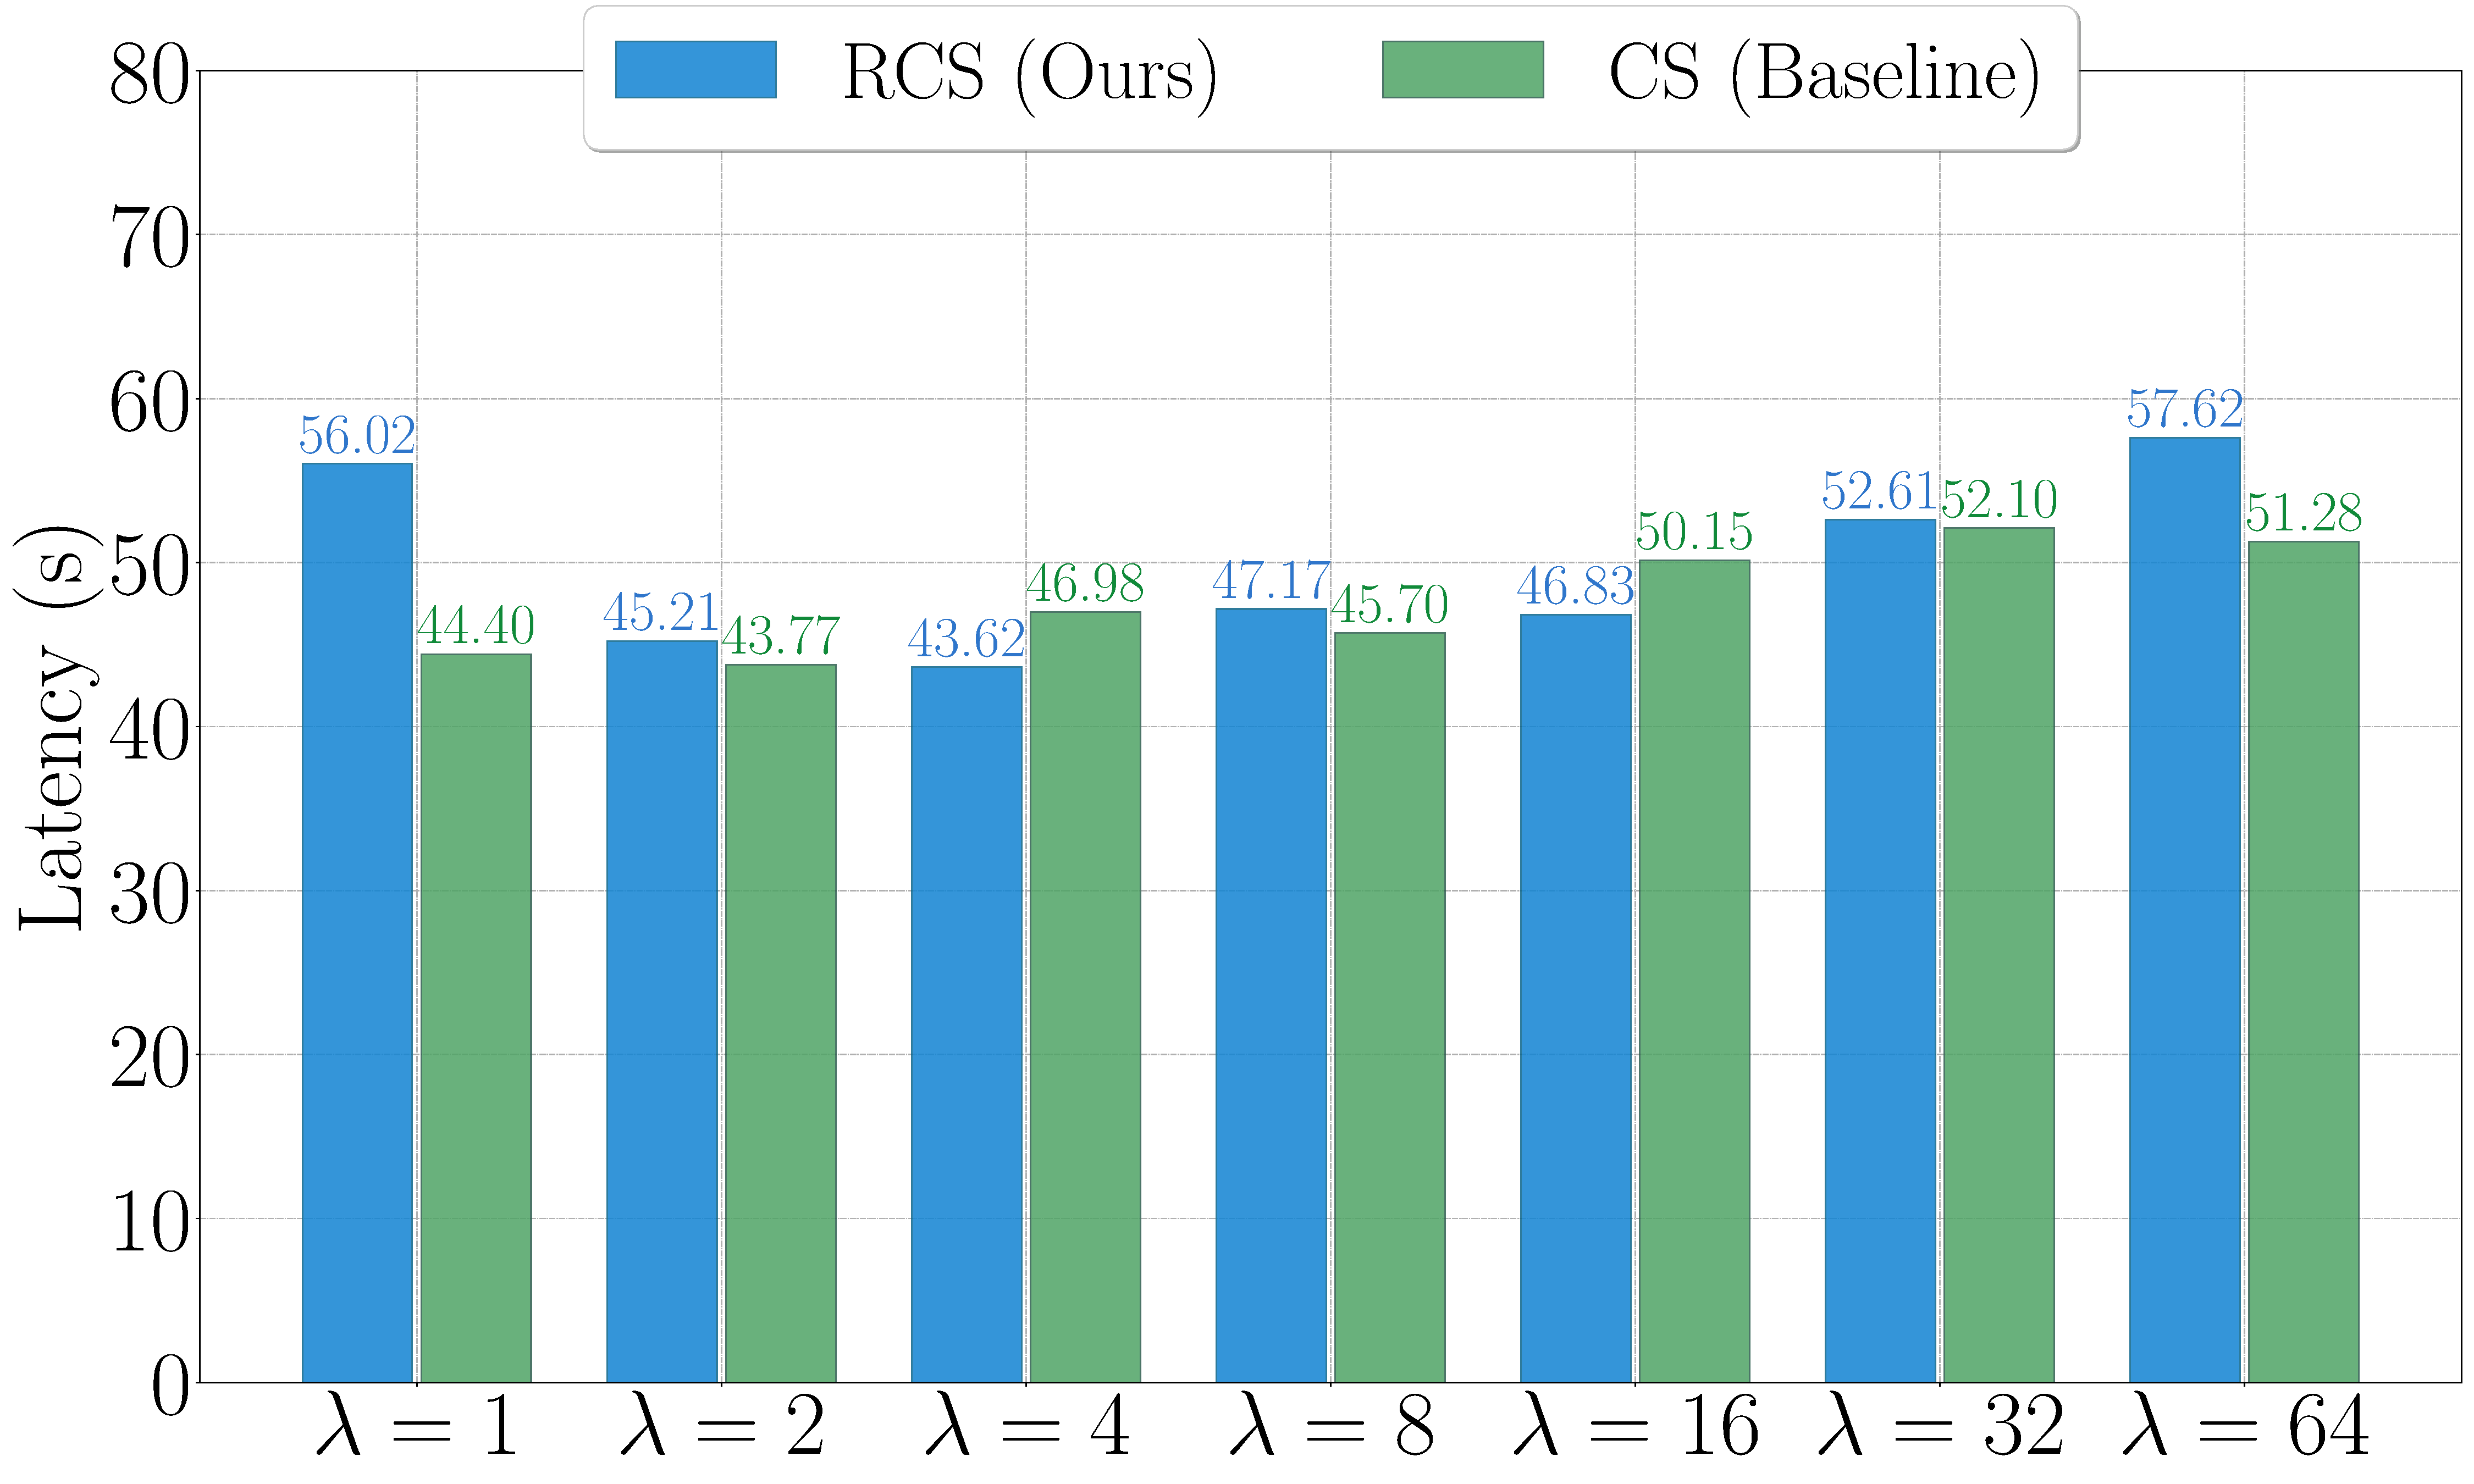
\includegraphics[width=\linewidth]{latex/eval_res/TC-129.pdf}
        \caption{$n=129$.}
    \end{subfigure}
    \caption{Evaluation results for the latency when $f < \lceil \frac{n}{2} \rceil$.}
    \label{fig:TC_g}
    % \vspace{-15pt}
\end{figure*}


\subsection{F-RCS Algorithm}
Based on the foundational theory in Section \ref{sec:Theory}, we construct an optimization algorithm for RCS, named Feedback-Optimized Reliable Consensus Sampling (F-RCS). In each sampling round, given the delivered response $y$ and the generating model $|\phi_r\rangle$, the algorithm identifies two additional models by a function $F(\cdot)$ (see Algorithm \ref{alg:F-RCS}). One model $|\phi_{\max}\rangle$ attains the maximum $p(y)$. Another model $|\phi_{\min}\rangle$ attains the minimum $p(y)$. If $y$ is judged unsafe at time $t$, then for subsequent similar tasks, $|\phi_{\max}\rangle$ is removed during random sampling. Formally, $\mathcal{MG} = \mathcal{MG} \setminus \{|\phi_{\max}\rangle\}.$ This allows, at the beginning of each algorithm execution, the system makes an automated decision. It selects safer models used in sampling for $x$. This process increases the safety margin $s - f$ and reduces risk. Here, $|\phi_{\max}\rangle$ can equal $|\phi_{r}\rangle$. Initially, $|\phi_{r}\rangle$ assigns the highest probability to $y$, which aligns with the algorithm objective. We call this behavior of model $|\phi_{r}\rangle$ self-entanglement. In addition, during sampling, the execution of the feedback algorithm is independent of RCS itself, and therefore does not affect the safety of RCS. For time overhead, the additional cost introduced by the feedback algorithm is negligible.



\begin{algorithm}[h]
\SetAlgoLined
\KwIn{
Parameters $(n, s, R)$;
evaluation method $a$
}
\KwOut{Response $y$}

\For{each prompt $x$}{
    $|\phi_{r}\rangle \gets F(x, \mathcal{MG})$ \\
    $\mathcal{MG}^{'} \gets \mathcal{MG} \setminus \{|\phi_{r}\rangle\}$ \\
    $\{y,\mathcal{P}\} \gets \text{RCS}(\mathcal{MG}^{'}, x, s, R)$ \\
    \textcolor{mGreen}{\#$\mathcal{P}=\{p_{|\phi_1\rangle}(y), \cdots, p_{|\phi_n\rangle}(y) \}$} \\
    \textcolor{mGreen}{\#Identify entangled models.} \\
    $|\phi_{\max}\rangle \gets \arg\max_{|\phi_i\rangle} p_{|\phi_i\rangle}(y)$ \\
    \textcolor{mGreen}{\#Record $<|\phi_{\max}\rangle\ ,x, y, |\phi_{r}\rangle>$.} \\
    \Return $y$ \\
    }
    
\While{time $t \in \mathbb{R}^{+}$}{
    \If{$|1\rangle \gets \mathrm{Eval}(x, |\phi_{r}\rangle, a)$}{
        New $F \gets \mathrm{Update}(F,|\phi_{\max}\rangle\ ,x)$ \\
    }
    $t \gets t + \Delta(t)$\\
}

\caption{F-RCS Algorithm}
\label{alg:F-RCS}
\end{algorithm}